% Build from the project root:
% latexmk -pdf -interaction=nonstopmode -halt-on-error -outdir=.scratch/presentation-build presentation.tex
% cp .scratch/presentation-build/presentation.pdf presentation.pdf
\documentclass[aspectratio=169,10pt]{beamer}

\usepackage[T1]{fontenc}
\usepackage{lmodern}
\usepackage{microtype}
\usepackage{amsmath,amssymb,bm}
\usepackage{tikz}
\usetikzlibrary{arrows.meta,positioning,calc}
\usepackage{booktabs}

% A light, restrained theme built directly on Beamer's defaults.
\definecolor{navy}{HTML}{17324D}
\definecolor{ink}{HTML}{243447}
\definecolor{muted}{HTML}{627386}
\definecolor{teal}{HTML}{137F82}
\definecolor{sea}{HTML}{2A9D8F}
\definecolor{blue}{HTML}{4677A8}
\definecolor{coral}{HTML}{E47755}
\definecolor{gold}{HTML}{D6A33D}
\definecolor{lilac}{HTML}{7A6FA8}
\definecolor{paper}{HTML}{F5F8FB}
\definecolor{mist}{HTML}{E8F2F3}
\definecolor{line}{HTML}{D9E3EC}

\setbeamercolor{normal text}{fg=ink,bg=white}
\setbeamercolor{structure}{fg=teal}
\setbeamercolor{frametitle}{fg=navy,bg=white}
\setbeamercolor{framesubtitle}{fg=muted}
\setbeamercolor{block title}{fg=white,bg=navy}
\setbeamercolor{block body}{fg=ink,bg=paper}
\setbeamercolor{block title alerted}{fg=white,bg=coral}
\setbeamercolor{block body alerted}{fg=ink,bg=coral!7}
\setbeamercolor{block title example}{fg=white,bg=teal}
\setbeamercolor{block body example}{fg=ink,bg=mist}
\setbeamercolor{card}{fg=ink,bg=paper}
\setbeamercolor{softcard}{fg=ink,bg=mist}
\setbeamercolor{takeaway}{fg=navy,bg=mist}
\setbeamercolor{placeholder}{fg=muted,bg=paper}
\setbeamercolor{footline}{fg=muted,bg=white}

\setbeamertemplate{navigation symbols}{}
\setbeamertemplate{itemize item}{\textcolor{teal}{\small$\blacksquare$}}
\setbeamertemplate{itemize subitem}{\textcolor{teal}{--}}
\setbeamertemplate{enumerate item}{\textcolor{teal}{\bfseries\insertenumlabel.}}
\setbeamersize{text margin left=9mm,text margin right=9mm}
\setbeamerfont{frametitle}{size=\Large,series=\bfseries}
\setbeamerfont{framesubtitle}{size=\small,series=\mdseries}
\setbeamerfont{footline}{size=\scriptsize}
\setlength{\leftmargini}{1.25em}

\setbeamertemplate{frametitle}{%
  \vspace*{3.0mm}%
  {\scriptsize\bfseries\color{teal}\insertsection\par}%
  \vspace{1.0mm}%
  {\usebeamerfont{frametitle}\color{navy}\insertframetitle\par}%
  \vspace{0.8mm}%
  {\usebeamerfont{framesubtitle}\color{muted}\insertframesubtitle\par}%
  \vspace{1.2mm}{\color{teal}\rule{13mm}{0.8pt}}\par\vspace{1.2mm}%
}

\setbeamertemplate{footline}{%
  \leavevmode%
  \hbox{%
    \begin{beamercolorbox}[wd=.79\paperwidth,ht=2.6ex,dp=1.15ex,leftskip=9mm]{footline}%
      \usebeamerfont{footline}From PDEs to butterfly factorisations
    \end{beamercolorbox}%
    \begin{beamercolorbox}[wd=.21\paperwidth,ht=2.6ex,dp=1.15ex,rightskip=9mm plus1fil]{footline}%
      \hfill\usebeamerfont{footline}\insertframenumber\,/\,\inserttotalframenumber
    \end{beamercolorbox}%
  }%
}

\newcommand{\pill}[2]{%
  \tikz[baseline=-0.65ex]\node[fill=#1!11,text=#1,rounded corners=2pt,
    inner xsep=5pt,inner ysep=2.6pt,font=\scriptsize\bfseries]{#2};%
}
\newcommand{\takeaway}[1]{%
  \begin{beamercolorbox}[rounded=true,sep=1.3ex]{takeaway}%
    \textcolor{teal}{\bfseries Takeaway}\quad #1
  \end{beamercolorbox}%
}
\newcommand{\draftnote}[1]{%
  \begin{beamercolorbox}[rounded=true,sep=1.3ex]{placeholder}%
    \textcolor{muted}{\bfseries Planned for this slide}\quad #1
  \end{beamercolorbox}%
}
\newcommand{\source}[1]{{\scriptsize\color{muted}#1\par}}

\title{From PDEs to butterfly factorisations}
\author{}
\date{}

\begin{document}

% 1 -----------------------------------------------------------------------
\begin{frame}[plain]
\begin{tikzpicture}[remember picture,overlay]
  \fill[navy] (current page.south west) rectangle (current page.north east);
  \fill[teal,opacity=.14] ([xshift=-4mm,yshift=2mm]current page.north east) circle (48mm);
  \fill[blue,opacity=.10] ([xshift=5mm,yshift=-4mm]current page.south east) circle (40mm);
  \draw[teal,line width=1.2mm] ([xshift=10mm,yshift=-15mm]current page.north west)
    -- ([xshift=10mm,yshift=-53mm]current page.north west);
  \node[anchor=north west,text=teal!55!white,font=\scriptsize\bfseries]
    at ([xshift=15mm,yshift=-16mm]current page.north west)
    {NUMERICAL METHODS FOR PDE INTEGRAL OPERATORS};
  \node[anchor=north west,text=white,text width=102mm,font=\fontsize{26}{31}\selectfont\bfseries]
    at ([xshift=15mm,yshift=-25mm]current page.north west)
    {From PDEs to\\butterfly factorisations};
  \node[anchor=north west,text=white!78,text width=89mm,font=\large]
    at ([xshift=15mm,yshift=-58mm]current page.north west)
    {Exploiting structure in Green-function\\and oscillatory integral operators};
  \node[anchor=south west,text=white!60,font=\small]
    at ([xshift=15mm,yshift=10mm]current page.south west)
    {20-minute presentation};

  \coordinate (bforigin) at ([xshift=-39mm,yshift=1mm]current page.east);
  \begin{scope}[shift=(bforigin),x=1mm,y=1mm]
    \foreach \x in {0,12,24,36}{
      \foreach \y in {-18,-6,6,18}{
        \fill[white!85] (\x,\y) circle (1.15);
      }
    }
    \foreach \a/\b in {-18/-18,-18/-6,-6/-18,-6/6,6/-6,6/18,18/6,18/18}
      \draw[teal!65!white,opacity=.75,line width=.55pt] (0,\a)--(12,\b);
    \foreach \a/\b in {-18/-18,-18/6,-6/-6,-6/18,6/-18,6/6,18/-6,18/18}
      \draw[white,opacity=.52,line width=.55pt] (12,\a)--(24,\b);
    \foreach \a/\b in {-18/-18,-18/-6,-6/-18,-6/6,6/-6,6/18,18/6,18/18}
      \draw[coral!80!white,opacity=.65,line width=.55pt] (24,\a)--(36,\b);
    \node[text=white!50,font=\scriptsize,align=center] at (18,-29)
      {local coefficients\\global interactions};
  \end{scope}
\end{tikzpicture}
\vspace*{0pt}
\end{frame}

\section{Roadmap}
% 2 -----------------------------------------------------------------------
\begin{frame}{One question, six steps}
\framesubtitle{How do we exploit the matrix structure inherited from PDEs?}
\small
\begin{columns}[T,onlytextwidth]
\column{.32\textwidth}
\begin{beamercolorbox}[rounded=true,sep=1.25ex]{softcard}
\pill{teal}{01 \quad MOTIVATION}\\[1mm]
{\bfseries PDEs and Green functions}\\
Continuous superposition $\rightarrow$ discrete matrix structure.
\end{beamercolorbox}
\vspace{2mm}
\begin{beamercolorbox}[rounded=true,sep=1.25ex]{card}
\pill{blue}{02 \quad FFT}\\[1mm]
{\bfseries Reusing computation}\\
Shared work gives $O(N\log N)$ instead of $O(N^2)$.
\end{beamercolorbox}
\column{.32\textwidth}
\begin{beamercolorbox}[rounded=true,sep=1.25ex]{card}
\pill{lilac}{03 \quad FACTORISATIONS}\\[1mm]
{\bfseries Interactions in stages}\\
Sparse factors and block-structured transformations.
\end{beamercolorbox}
\vspace{2mm}
\begin{beamercolorbox}[rounded=true,sep=1.25ex]{softcard}
\pill{teal}{04 \quad BUTTERFLY}\\[1mm]
{\bfseries Oscillatory integrals}\\
Centred phases and complementary low-rank blocks.
\end{beamercolorbox}
\column{.32\textwidth}
\begin{beamercolorbox}[rounded=true,sep=1.25ex]{card}
\pill{blue}{05 \quad LINEAR ALGEBRA}\\[1mm]
{\bfseries The matrix viewpoint}\\
Multilevel recursions as products of sparse factors.
\end{beamercolorbox}
\vspace{2mm}
\begin{beamercolorbox}[rounded=true,sep=1.25ex]{card}
\pill{muted}{06 \quad DISCUSSION}\\[1mm]
{\bfseries Scope and limitations}\\
Accuracy, applicability and fast application versus solution.
\end{beamercolorbox}
\end{columns}
\end{frame}

\section{1 \textbar\quad Motivation: PDEs and Green functions}
% 3 -----------------------------------------------------------------------
\begin{frame}{Green functions turn PDEs into matrix problems}
\framesubtitle{Discretisation preserves structure inherited from the continuous operator.}
\begin{columns}[T,onlytextwidth]
\column{.57\textwidth}
{\color{teal}\small\bfseries CONTINUOUS SUPERPOSITION}
\[
 \mathcal Lu=f
 \quad\Longrightarrow\quad
 u(x)=\int_\Omega G(x,y)f(y)\,\mathrm dy .
\]
{\small $G(x,y)$ is the effect at $x$ of a unit point source at $y$.}
\vspace{2mm}

{\color{teal}\small\bfseries DISCRETE SUPERPOSITION}
\[
 u(x_i)\approx\sum_{j=1}^{N}\underbrace{w_jG(x_i,y_j)}_{A_{ij}}\,f(y_j)
 \quad\Longrightarrow\quad \bm u=A\bm f .
\]
{\small Quadrature points $y_j$, observations $x_i$ and weights $w_j$ determine the matrix entries.}
\column{.39\textwidth}
\begin{block}{Apply a known operator}
Given $f$, compute $\bm u=A\bm f$.\\[.5ex]
\textbf{Task:} fast matrix--vector multiplication.
\end{block}
\vspace{2mm}
\begin{alertblock}{Solve for an unknown density}
Given $b$, compute $\bm\sigma$ from $A\bm\sigma=b$.\\[.5ex]
\textbf{Fast application of $A$ does not automatically give a fast direct solver.}
\end{alertblock}
\end{columns}
\end{frame}

% 4 -----------------------------------------------------------------------
\begin{frame}{Three PDE examples, three kinds of matrix structure}
\framesubtitle{Diagonal apply $\rightarrow$ oscillatory apply $\rightarrow$ dense oscillatory solve.}
\small
\begin{columns}[T,onlytextwidth]
\column{.315\textwidth}
\begin{beamercolorbox}[rounded=true,sep=1.1ex]{softcard}
\pill{teal}{HEAT \quad PERIODIC}\\[1mm]
{\bfseries Fourier modes decouple}\\[.7mm]
{\footnotesize$\widehat u_m(t)=e^{-4\pi^2\kappa m^2t}\widehat u_{0,m}$}
\begin{center}
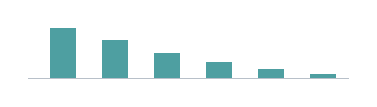
\begin{tikzpicture}[x=.55mm,y=.40mm,baseline]
 \draw[muted!45] (0,0)--(74,0);
 \foreach \x/\h in {5/16,17/12,29/8,41/5,53/2.8,65/1.2}
   \fill[teal!75] (\x,0) rectangle ++(6,\h);
\end{tikzpicture}
\end{center}
{\scriptsize\textbf{Structure:} diagonal in Fourier space; circulant on a uniform periodic grid.\\[.7mm]
\textbf{Computation:} independent scalar multipliers; damping smooths high frequencies.}
\end{beamercolorbox}
\column{.315\textwidth}
\begin{beamercolorbox}[rounded=true,sep=1.1ex]{card}
\pill{blue}{WAVE \quad PERIODIC}\\[1mm]
{\bfseries Phases remain active}\\[.7mm]
{\footnotesize$\Phi_\pm(x,m)=m\cdot x\pm ct|m|$}
\begin{center}
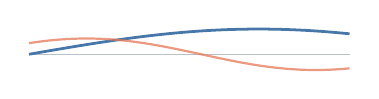
\begin{tikzpicture}[x=.55mm,y=.40mm,baseline]
 \draw[muted!45] (0,0)--(74,0);
 \draw[blue,line width=1pt] plot[domain=0:74,samples=90] (\x,{8*sin(\x*1.7)});
 \draw[coral,line width=.8pt,opacity=.75] plot[domain=0:74,samples=90] (\x,{5*sin(\x*3.4+45)});
\end{tikzpicture}
\end{center}
{\scriptsize\textbf{Structure:} an oscillatory Fourier integral operator.\\[.7mm]
\textbf{Computation:} unit-modulus multipliers keep modes active; this special periodic problem remains diagonalisable.}
\end{beamercolorbox}
\column{.315\textwidth}
\begin{beamercolorbox}[rounded=true,sep=1.1ex]{card}
\pill{coral}{HELMHOLTZ \quad SCATTERING}\\[1mm]
{\bfseries A dense system to solve}\\[.7mm]
{\footnotesize$G_k(x,y)=\dfrac{e^{ik|x-y|}}{4\pi|x-y|}$}
\begin{center}
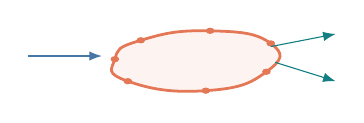
\begin{tikzpicture}[x=.55mm,y=.40mm,baseline]
 \draw[coral,fill=coral!8,line width=1pt] plot[smooth cycle,tension=.9]
   coordinates {(25,2)(43,-1)(57,5)(58,14)(44,18)(28,15)(22,9)};
 \foreach \p in {(25,2),(43,-1),(57,5),(58,14),(44,18),(28,15),(22,9)}
   \fill[coral] \p circle (1);
 \draw[blue,-{Latex[length=1.6mm]}] (2,10)--(19,10);
 \draw[teal,-{Latex[length=1.6mm]}] (59,8)--(73,2);
 \draw[teal,-{Latex[length=1.6mm]}] (58,13)--(73,17);
\end{tikzpicture}
\end{center}
{\scriptsize\textbf{Structure:} dense, oscillatory and singular on a general boundary.\\[.7mm]
\textbf{Computation:} solve $A\sigma=b$ for the density, then evaluate the scattered field.}
\end{beamercolorbox}
\end{columns}
\end{frame}

\section{2 \textbar\quad The FFT}
% 5 -----------------------------------------------------------------------
\begin{frame}{Why $O(N\log N)$ instead of $O(N^2)$?}
\framesubtitle{Section 2 placeholder: the FFT is the prototype for reusing intermediate work.}
\pill{blue}{SECTION 2 \quad TO BE COMPLETED}
\vspace{2mm}
\begin{columns}[T,onlytextwidth]
\column{.40\textwidth}
\draftnote{Add one even/odd split and connect its recurrence to the diagram.}
\[
\begin{gathered}
 T(N)=2T(N/2)+O(N),\\
 T(N)=O(N\log N).
\end{gathered}
\]
{\scriptsize\color{muted}\textbf{Message:} exact reuse, not approximation.}
\column{.55\textwidth}
\begin{center}
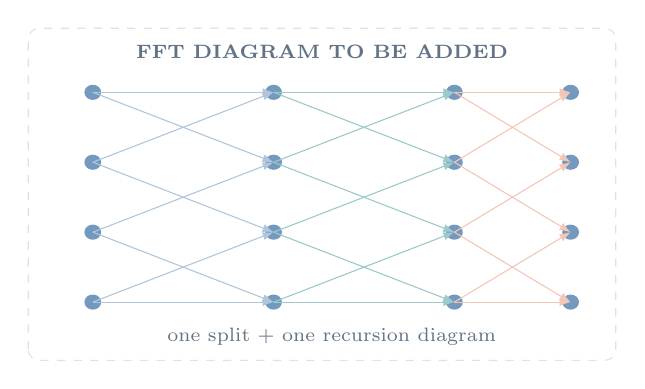
\begin{tikzpicture}[x=.82mm,y=.74mm]
 \draw[dashed,draw=line,rounded corners] (0,-28) rectangle (91,29);
 \node[font=\scriptsize\bfseries,text=muted] at (45.5,25){FFT DIAGRAM TO BE ADDED};
 \foreach \x in {10,38,66,84}
   \foreach \y in {-18,-6,6,18}{\fill[blue!75] (\x,\y) circle (1.3);}
 \foreach \a/\b in {-18/-18,-18/-6,-6/-18,-6/6,6/-6,6/18,18/6,18/18}{
   \draw[blue!42,-{Latex[length=1.4mm]}] (10,\a)--(38,\b);
   \draw[teal!42,-{Latex[length=1.4mm]}] (38,\a)--(66,\b);
   \draw[coral!42,-{Latex[length=1.4mm]}] (66,\a)--(84,\b);
 }
 \node[font=\scriptsize,text=muted] at (47,-24){one split + one recursion diagram};
\end{tikzpicture}
\end{center}
\end{columns}
\end{frame}

\section{3 \textbar\quad General factorisations}
% 6 -----------------------------------------------------------------------
\begin{frame}{A factorisation reorganises interactions}
\framesubtitle{Section 3 placeholder: connect the FFT picture to block-structured matrices.}
\pill{lilac}{SECTION 3 \quad TO BE COMPLETED}
\vspace{2mm}
\begin{columns}[T,onlytextwidth]
\column{.44\textwidth}
\draftnote{Define factorisation as a sequence of manageable stages. Distinguish exact sparsity from numerical low rank.}
\vspace{2mm}
\begin{beamercolorbox}[rounded=true,sep=1.3ex]{card}
{\bfseries Three ideas to define}\\[.7mm]
{\scriptsize Sparse factors\\[.4mm] Block interactions\\[.4mm] Compression without discarding contributions}
\end{beamercolorbox}
\column{.51\textwidth}
\begin{center}
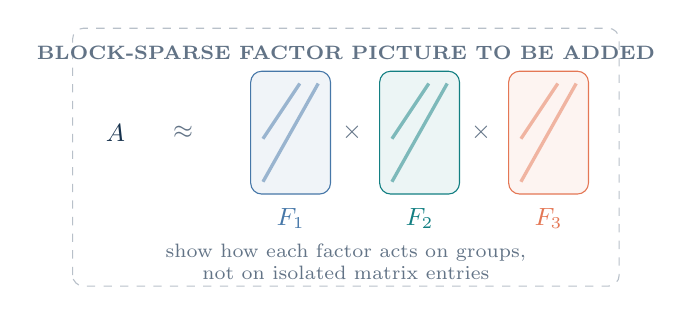
\begin{tikzpicture}[x=.78mm,y=.78mm]
 \node[font=\small\bfseries,text=navy] (A) at (0,13) {$A$};
 \node[font=\small,text=muted] at (11,13) {$\approx$};
 \foreach \x/\c/\lab in {22/blue/{$F_1$},43/teal/{$F_2$},64/coral/{$F_3$}}{
   \draw[fill=\c!8,draw=\c,rounded corners] (\x,3) rectangle ++(13,20);
   \draw[\c!55,line width=1.2pt] (\x+2,5)--(\x+11,21);
   \draw[\c!55,line width=1.2pt] (\x+2,12)--(\x+8,21);
   \node[font=\small,text=\c] at (\x+6.5,-1) {\lab};
   \ifnum\x<64 \node[font=\small,text=muted] at (\x+16.5,13) {$\times$};\fi
 }
 \draw[dashed,muted!45,rounded corners] (-7,-12) rectangle (82,30);
 \node[font=\scriptsize\bfseries,text=muted] at (37.5,26){BLOCK-SPARSE FACTOR PICTURE TO BE ADDED};
 \node[font=\scriptsize,text=muted,align=center] at (37.5,-8)
   {show how each factor acts on groups,\\not on isolated matrix entries};
\end{tikzpicture}
\end{center}
\end{columns}
\end{frame}

\section{4 \textbar\quad Butterfly factorisation}
% 7 -----------------------------------------------------------------------
\begin{frame}{Remove the large phase exactly; approximate only the residual}
\framesubtitle{On a rectangle $A\times B$, centre the phase at $(a,b)$.}
\small
\begin{columns}[T,onlytextwidth]
\column{.68\textwidth}
\vspace{-2mm}
\[
\begin{aligned}
 K_n(x,p)&=e^{2\pi i n\Psi(x,p)},\\
 R_{AB}&=\Psi(x,p)-\Psi(a,p)-\Psi(x,b)+\Psi(a,b).
\end{aligned}
\]
\begin{beamercolorbox}[rounded=true,sep=1.0ex]{softcard}
\centering
\resizebox{\linewidth}{!}{$\displaystyle K_n=\underbrace{e^{2\pi in\Psi(x,b)}}_{x\ \mathrm{only}}\,
 \underbrace{e^{2\pi in\Psi(a,p)}}_{p\ \mathrm{only}}\,
 \underbrace{e^{-2\pi in\Psi(a,b)}}_{\mathrm{constant}}\,
 \underbrace{e^{2\pi inR_{AB}}}_{\mathrm{coupled\ residual}}$}
\end{beamercolorbox}
\vspace{1mm}
\[
\begin{aligned}
 R_{AB}(x,p)&=\int_a^x\!\int_b^p\partial_s\partial_t\Psi(s,t)\,\mathrm dt\,\mathrm ds,\\
 2\pi n|R_{AB}|&\leq\rho_{AB}
 :=\frac{\pi}{2}M_{AB}\,n h_Ah_B,
 \qquad M_{AB}=\sup_{A\times B}|\partial_x\partial_p\Psi|.
\end{aligned}
\]\column{.27\textwidth}
\begin{center}
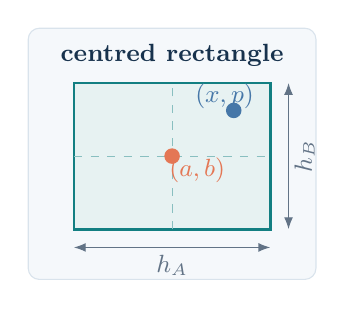
\begin{tikzpicture}[x=.58mm,y=.58mm]
 \draw[fill=paper,draw=line,rounded corners] (0,-3) rectangle (63,52);
 \draw[fill=teal!10,draw=teal,line width=1pt] (10,8) rectangle (53,40);
 \draw[teal!50,dashed] (31.5,8)--(31.5,40);
 \draw[teal!50,dashed] (10,24)--(53,24);
 \fill[coral] (31.5,24) circle (1.7);
 \node[font=\small,text=coral] at (37,21){$(a,b)$};
 \fill[blue] (45,34) circle (1.7);
 \node[font=\small,text=blue] at (43,37){$(x,p)$};
 \draw[{Latex[length=1.5mm]}-{Latex[length=1.5mm]},muted] (10,4)--(53,4);
 \node[font=\small,text=muted] at (31.5,0){$h_A$};
 \draw[{Latex[length=1.5mm]}-{Latex[length=1.5mm]},muted] (57,8)--(57,40);
 \node[font=\small,text=muted,rotate=90] at (60.5,24){$h_B$};
 \node[font=\small\bfseries,text=navy] at (31.5,46){centred rectangle};
\end{tikzpicture}
\end{center}
\end{columns}
\vspace{.5mm}
\source{Cand\`es--Demanet--Ying, arXiv:0809.0719, \S\S3--4.}
\end{frame}

% 8 -----------------------------------------------------------------------
\begin{frame}{A small residual phase yields a short separated expansion}
\framesubtitle{After discretisation, a sum of $q$ separated terms is a block of rank at most $q$.}
\footnotesize
\begin{columns}[T,onlytextwidth]
\column{.51\textwidth}
\begin{block}{Bilinear model: $\Psi(x,p)=xp$}
Here $R_{AB}=(x-a)(p-b)$, and
\vspace{-1mm}
\[
\begin{aligned}
 e^{2\pi inR}&=\sum_{r=0}^{q-1}
 \frac{(2\pi in)^r}{r!}(x-a)^r(p-b)^r+\mathcal E_q,\\
 |\mathcal E_q|&\leq\frac{\rho_{AB}^q}{q!}.
\end{aligned}
\]
Every term is separated; the three remaining factors preserve rank and error.
\end{block}
\column{.43\textwidth}
\begin{exampleblock}{General real-analytic phase}
Chebyshev-interpolate $e^{2\pi inR_{AB}}$ in the smaller box's variable.
\begin{center}
\color{teal}\bfseries\scriptsize
prefactor $\rightarrow$ interpolate $\rightarrow$ remodulate
\end{center}
For $h_Ah_B=1/n$, the two-dimensional theorem gives $r_\varepsilon=O(\log^4(1/\varepsilon))$, with constant independent of $n$ in its range.
\end{exampleblock}
\end{columns}
\vspace{1mm}
{\scriptsize\color{muted}\textbf{Caveat:} the factorial bound is bilinear-specific; propagated multilevel errors need a separate estimate.}
\end{frame}

% 9 -----------------------------------------------------------------------
\begin{frame}{Complementary boxes keep the residual bound constant}
\framesubtitle{Refine observation boxes while coarsening source boxes: the width product never changes.}
\footnotesize
\begin{columns}[T,onlytextwidth]
\column{.55\textwidth}
At level $\ell$ of a depth-$L$ dyadic tree, $L=\log_2 n$,
\[
 A_\ell:\ h_\ell=2^{-\ell},\qquad
 B_{L-\ell}:\ H_\ell=2^\ell/n,
 \qquad\boxed{h_\ell H_\ell=1/n.}
\]
If $M$ uniformly bounds $|\partial_x\partial_p\Psi|$, then
\[
 \rho_\ell\leq\frac{\pi}{2}Mnh_\ell H_\ell
 =\frac{\pi}{2}M
 \qquad\text{at every level}.
\]
\takeaway{Complementary levels keep $n h_\ell H_\ell=1$: uniform residual bounds and, for analytic phases, uniform local rank targets.}
\column{.40\textwidth}
\begin{center}
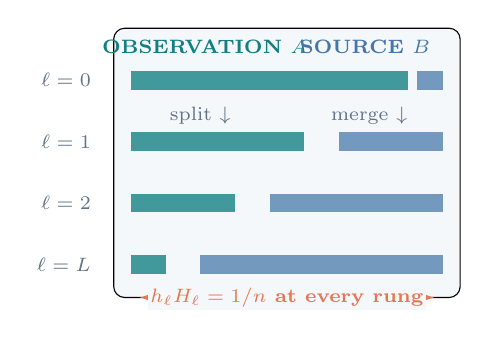
\begin{tikzpicture}[x=.55mm,y=.60mm]
 \draw[fill=paper,rounded corners] (-4,-9) rectangle (76,48);
 \node[font=\scriptsize\bfseries,text=teal] at (17,44){OBSERVATION $A$};
 \node[font=\scriptsize\bfseries,text=blue] at (54,44){SOURCE $B$};
 \foreach \y/\a/\b/\lab in {35/64/6/{$\ell=0$},22/40/24/{$\ell=1$},9/24/40/{$\ell=2$},-4/8/56/{$\ell=L$}}{
   \node[font=\scriptsize,text=muted,anchor=east] at (-7,\y+2){\lab};
   \fill[teal!80] (0,\y) rectangle ++(\a,4);
   \fill[blue!75] (72-\b,\y) rectangle ++(\b,4);
 }
 \node[font=\scriptsize,text=muted] at (16,29.5){split $\downarrow$};
 \node[font=\scriptsize,text=muted] at (55,29.5){merge $\downarrow$};
 \draw[{Latex[length=1.5mm]}-{Latex[length=1.5mm]},coral] (2,-9)--(70,-9);
 \node[font=\scriptsize\bfseries,text=coral,fill=paper,inner sep=1pt] at (36,-9){$h_\ell H_\ell=1/n$ at every rung};
\end{tikzpicture}
\end{center}
\vspace{1mm}
{\scriptsize $n$ pairs per level; $O(n\log n)$ total.}
\end{columns}
\end{frame}

% 10 ----------------------------------------------------------------------
\begin{frame}{Compressed potentials become a multilevel butterfly recursion}
\framesubtitle{Complementary low-rank blocks and short coefficient transfers produce multilevel reuse.}
\small
\begin{columns}[T,onlytextwidth]
\column{.39\textwidth}
\begin{block}{One complementary block}
\footnotesize
\[
\begin{aligned}
 u_B(x)&\approx\sum_{t=1}^{r}\alpha_t^{AB}(x)\,\delta_t^{AB},\\
 \delta_t^{AB}&=\sum_{p_j\in B}\beta_t^{AB}(p_j)f(p_j).
\end{aligned}
\]
Only $r$ coefficients represent all sources in $B$ throughout observation box $A$.
\end{block}
\column{.31\textwidth}
\begin{center}
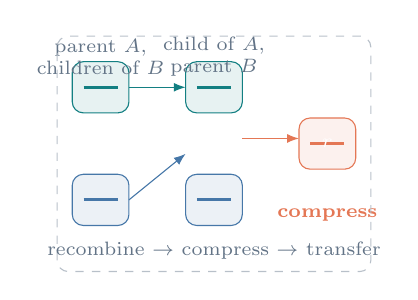
\begin{tikzpicture}[x=.48mm,y=.65mm,node distance=0pt]
 \foreach \x/\y/\c in {0/32/teal,0/10/blue,30/32/teal,30/10/blue,60/21/coral}{
   \draw[fill=\c!10,draw=\c,rounded corners] (\x,\y) rectangle ++(15,10);
   \draw[\c,line width=1pt] (\x+3,\y+5)--(\x+12,\y+5);
 }
 \node[font=\scriptsize,text=muted,align=center] at (7.5,43){parent $A$,\\children of $B$};
 \node[font=\scriptsize,text=muted,align=center] at (37.5,43){child of $A$,\\parent $B$};
 \draw[teal,-{Latex[length=1.5mm]}] (15,37)--(30,37);
 \draw[blue,-{Latex[length=1.5mm]}] (15,15)--(30,24);
 \draw[coral,-{Latex[length=1.5mm]}] (45,27)--(60,27);
 \node[font=\scriptsize,text=white] at (67.5,26){$r$};
 \node[font=\scriptsize\bfseries,text=coral] at (67.5,12){compress};
 \draw[dashed,muted!45,rounded corners] (-4,1) rectangle (79,47);
 \node[font=\scriptsize,text=muted] at (37.5,5){recombine $\rightarrow$ compress $\rightarrow$ transfer};
\end{tikzpicture}
\end{center}
\column{.25\textwidth}
\begin{beamercolorbox}[rounded=true,sep=1.2ex]{softcard}
{\bfseries Fixed local rank}\\[.7mm]
{\scriptsize $n$ pairs per level; $L+1$ levels.\\[.7mm]
\textbf{1D:} $O(n\log n)$ updates.\\[.7mm]
\textbf{2D quadtree:} $O(N^2\log N)$.}
\end{beamercolorbox}
\end{columns}
\end{frame}

\section{5 \textbar\quad Numerical linear algebra}
% 11 ----------------------------------------------------------------------
\begin{frame}{Butterfly factorisation as numerical linear algebra}
\framesubtitle{Section 5 placeholder: make the sparse-factor formulation explicit.}
\pill{blue}{SECTION 5 \quad TO BE COMPLETED}
\vspace{2mm}
\begin{columns}[T,onlytextwidth]
\column{.44\textwidth}
\draftnote{Add explicit sparse factors, block dimensions, rank choices and error bookkeeping.}
\vspace{1mm}
\begin{beamercolorbox}[rounded=true,sep=1.3ex]{card}
{\bfseries Two comparisons to add}\\[.7mm]
{\scriptsize Residual interpolation versus SVD/ID constructions.\\[.6mm]
Fast operator application versus direct solution of a linear system.}
\end{beamercolorbox}
\column{.51\textwidth}
\begin{center}
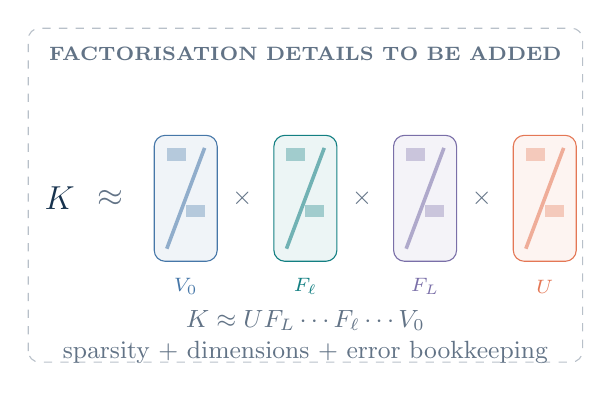
\begin{tikzpicture}[x=.8mm,y=.8mm]
 \draw[dashed,muted!45,rounded corners] (-3,-16) rectangle (85,37);
 \node[font=\scriptsize\bfseries,text=muted] at (41,33){FACTORISATION DETAILS TO BE ADDED};
 \node[font=\large,text=navy] at (2,10){$K$};
 \node[font=\large,text=muted] at (10,10){$\approx$};
 \foreach \x/\c/\lab in {17/blue/{$V_0$},36/teal/{$F_\ell$},55/lilac/{$F_L$},74/coral/{$U$}}{
   \draw[fill=\c!8,draw=\c,rounded corners] (\x,0) rectangle ++(10,20);
   \draw[\c!60,line width=1.3pt] (\x+2,2)--(\x+8,18);
   \fill[\c!40] (\x+2,16) rectangle ++(3,2);
   \fill[\c!40] (\x+5,7) rectangle ++(3,2);
   \node[font=\scriptsize,text=\c] at (\x+5,-4){\lab};
   \ifnum\x<74 \node[font=\small,text=muted] at (\x+14,10){$\times$};\fi
 }
 \node[font=\small,text=muted,align=center] at (41,-12)
   {$K\approx U F_L\cdots F_\ell\cdots V_0$\\sparsity + dimensions + error bookkeeping};
\end{tikzpicture}
\end{center}
\end{columns}
\end{frame}

\section{6 \textbar\quad Discussion and limitations}
% 12 ----------------------------------------------------------------------
\begin{frame}{Where the structure helps---and where it can break}
\framesubtitle{Section 6 placeholder: close with the scope of the method, not just its operation count.}
\pill{muted}{SECTION 6 \quad TO BE EXPANDED}
\vspace{2mm}
\footnotesize
\begin{columns}[T,onlytextwidth]
\column{.31\textwidth}
\begin{beamercolorbox}[rounded=true,sep=1.2ex]{softcard}
\pill{teal}{WHAT ENABLES SPEED}\\[1mm]
\begin{itemize}
 \item Complementary low-rank blocks with frequency-independent local rank targets.
 \item Multilevel reuse of short coefficient vectors.
\end{itemize}
\vspace{-2mm}
\end{beamercolorbox}
\column{.31\textwidth}
\begin{beamercolorbox}[rounded=true,sep=1.2ex]{card}
\pill{coral}{WHAT NEEDS CARE}\\[1mm]
\begin{itemize}
 \item Higher derivatives, singularities and non-analytic phases.
 \item Rank--accuracy trade-offs and global error propagation.
 \item Variable media without a suitable global FIO form.
\end{itemize}
\vspace{-2mm}
\end{beamercolorbox}
\column{.31\textwidth}
\begin{beamercolorbox}[rounded=true,sep=1.2ex]{card}
\pill{blue}{WHAT REMAINS DISTINCT}\\[1mm]
\begin{itemize}
 \item Fast application $\neq$ fast direct solution.
 \item General butterfly machinery $\neq$ faster wall time than a specialised FFT.
 \item Local low rank $\neq$ a low-rank full matrix.
\end{itemize}
\vspace{-2mm}
\end{beamercolorbox}
\end{columns}
\vspace{1mm}
\begin{beamercolorbox}[rounded=true,sep=1.2ex]{takeaway}
\centering\bfseries
Speed comes from preserving and reorganising interactions---\\neither treating them as unrelated nor simply throwing them away.
\end{beamercolorbox}
\end{frame}

\end{document}
